\documentclass[titlepage]{article}
\usepackage{Preamble}


\title{ColSim: A Monte-Carlo event generator for proton-proton collisions \\[8pt] Milestone 4: Model Implementation: UML Diagram UPDATE \\[5pt] CS 4632: Modeling and Simulation}
\author{Casey Hampson}

\begin{document}
\maketitle
\pagebreak

\section*{UML Diagram and Initial Design Documentation}

\begin{figure}[ht]
  \centering
  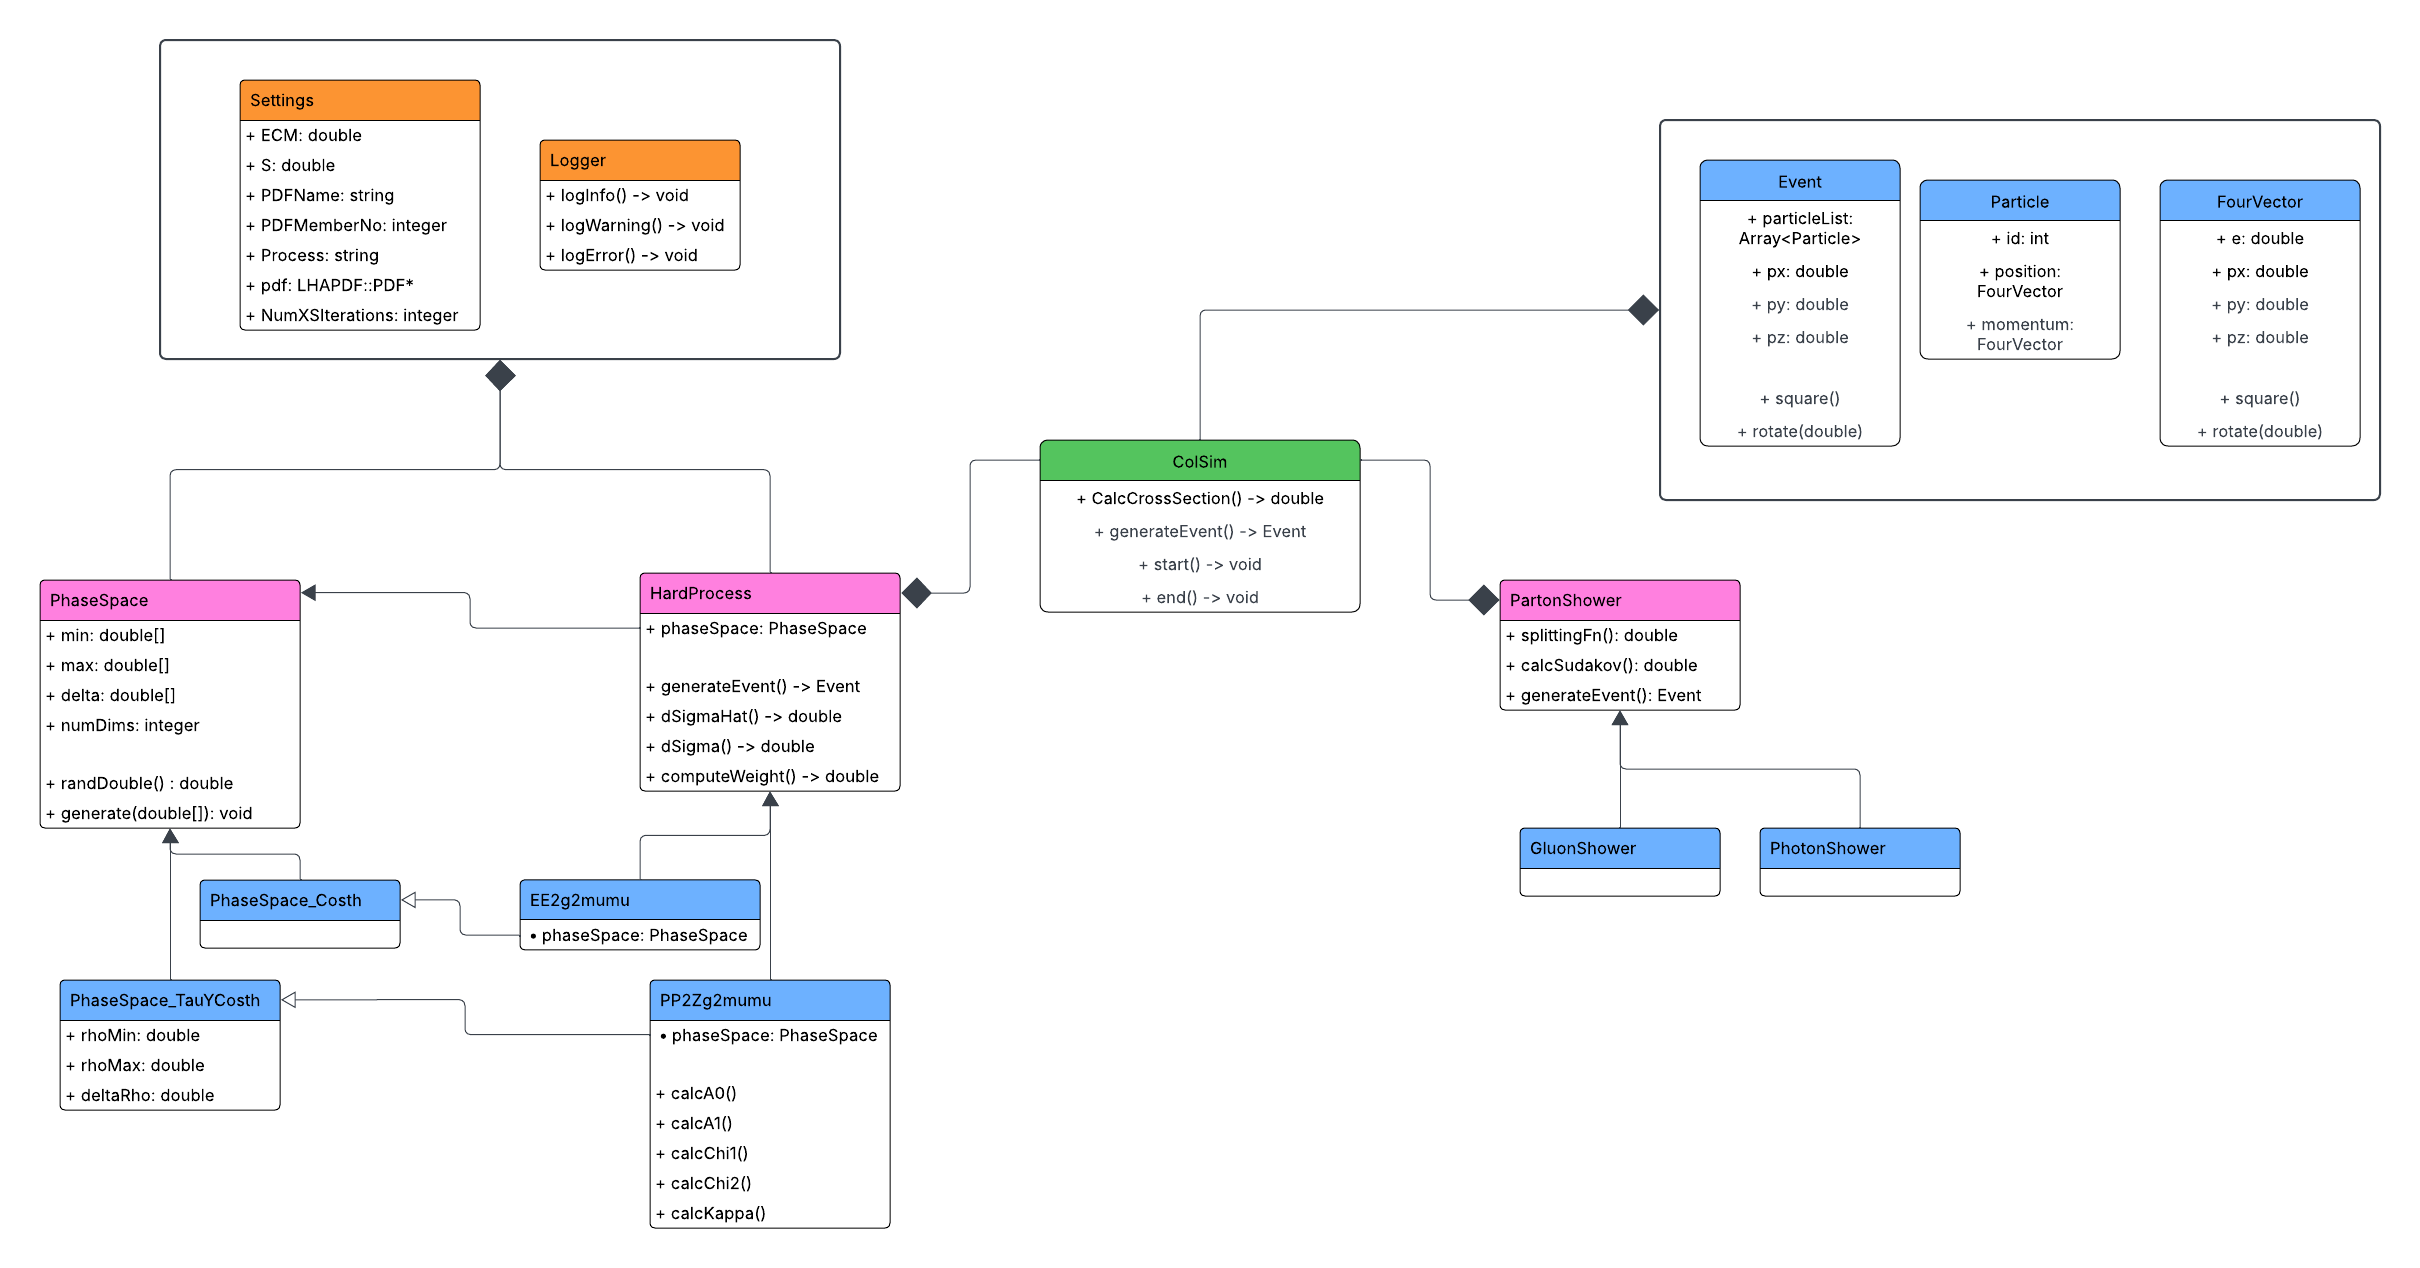
\includegraphics[width=0.9\linewidth]{./res/ColSim.png}
  \caption{UML diagram for ColSim.}
  \label{fig:uml}
\end{figure}

\subsection*{Description of Graphical Elements}

Here is a brief description of what the various graphical elements mean:

\begin{itemize}
\item \textit{Orange blocks}: Singleton classes. These are global/static classes whose data/methods are meant to be accessed at any point in the program.
\item \textit{Pink blocks}: Base classes used to group common behavior for the various types of processes.
\item \textit{Blue blocks}: Classes that are meant to be instantiated and contain behavior relevent to the specific process it represents.
\item \textit{Green block}: This is the main class that interfaces with the other classes. In particular, it does this in a general way via polymorphism, i.e. the user determines the hard process but all the code in this class needs to do is call the \mintinline{cpp}{dSigma()} method to get the differential cross section, from which it can do the Monte Carlo integration and determine the total cross section.
\item \textit{Solid arrow}: The solid arrow indicates direct object-oriented inheritance, or as a way to indicate a direct data type/relation. As an example of the latter, the \mintinline{cpp}{HardProcess} base class contains a \mintinline{cpp}{PhaseSpace} pointer that is inherited by its subclasses, so a solid arrow is drawn from that member to the \mintinline{cpp}{PhaseSpace} class to indicate this relationship.
\item \textit{Open arrow}: The open arrow is used to indicate relationships similar to those indicated by the solid arrow, but for subclasses. Just as the base hard process class has a phase space data member, each hard process subclass instantiates a phase space subclass; an open arrow points from this member to the phase space subclass.
\item \textit{Solid diamond}: The solid diamond indicates a dependence, but not one inherently tied to object-oriented behavior or as a direct member of a class. All classes use the functionality present in the \mintinline{cpp}{Settings} and \mintinline{cpp}{Logger} classes for instance, but since no instantiation is made nor do any other classes contain any instances of these classes, this uses a different symbol.
\end{itemize}


\subsection*{Description of Model and UML Diagram}

The main ``entry point'' to using ColSim is from the main \mintinline{cpp}{ColSimMain} class, which, as signified by the solid diamond connections, uses functionality from both the \mintinline{cpp}{HardProcess} and \mintinline{cpp}{PartonShower} classes, but does not directly dependend/inheret from them from an object-oriented point of view. By providing values in the configuration file whose data is available in the \mintinline{cpp}{Settings} class (which is thus available to the rest of the program), the first half of the program will compute the cross section and generate events at the hard process level. It will then pass these to the parton showering part of the program from which it will continue generating further events. 

\subsubsection*{The Hard Process}

The basic structure in place for the hard process calculations and event generators are done in a generic way in preparation for multiple different processes to be implemented. The main \mintinline{cpp}{HardProcess} class contains a pointer to a \mintinline{cpp}{PhaseSpace} object, and subclasses instantiate it with a reference to a derived phase space type. The phase space functionality is used to essentially define the independent variables for the integration associated with the cross section of a particular process. For instance, the integration for the process $qq \rightarrow Z\gamma \rightarrow \ell^+\ell^-$ includes the variables $\tau$, $y$, and $\cos\theta$, and it is this derived phase space class that this process instantiates. Similarly, if the initial state is replaced with two electrons rather than two quarks, the phase space is reduced to simply $\cos\theta$, and so it is this derived phase space class this process instantiates.

The main class, as described earlier, will instantiate the corresponding derived hard process class as a pointer to the base class, from which we can simply called any base method, and pass any results to the parton showering part of the program without bothering with any of the specifics that are all contained within the hard process classes themselves.

\subsubsection*{The Parton Showering}

This part of the program is structured exactly the same as the hard process component. The parton showering process is defined by the Sudakov form factor (as described in Milestone 2), as well as functions called \textit{splitting functions} which are related to the Sudakov factor and roughly correspond to the probability a parton (e.g. a quark or electron) will radiate a photon or gluon. The base \mintinline{cpp}{PartonShowering} process defines this behavior and different showering types implement the specific behavior themselves.

Then, just like in the other case, the user defines settings in the configuration file corresponding to the desired showering type (and other required parameters), and the main class can handle this in a general way.

\subsubsection*{Singleton and Other Utility Class}

There are not many specifics behind the singleton/utility classes apart from the fact that they provide a global instance to the entire program for things that should be, well, global. For instance, any part of the program should be able to log output to standard out/err and/or a file for error/warning reporting, for instance. The \mintinline{cpp}{Logger} class handles this; in particular it handles the file stream(s) and formatting of the output to appear nicer and contain information like the time it was logged, colors (if the user's terminal supports colors), as well as where in the code the message was logged.

Additionally, the \mintinline{cpp}{Settings} class contains information the user specifies in the configuration file. The center-of-mass energy of the hard scattering process is a parameter that is relevant in nearly every part of the program, so having it be easily available to all of the classes is important.


\end{document}
